% !TEX root = ../thesis.tex
%
\chapter{Pipeline}
\label{sec:pipeline}

\section{Training}
\label{sec:pipeline:training}
\subsection{Preprocessing and augmentation}
\label{sec:pipeline:training:augment}
\begin{figure}[htb]
    \begin{tabularx}{\textwidth}{XXXXX}
        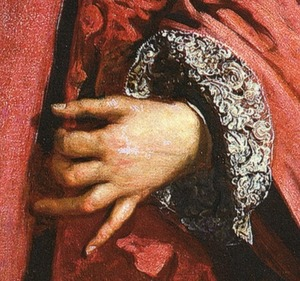
\includegraphics[width=0.170\textwidth]{figures/build/parts_example} &
        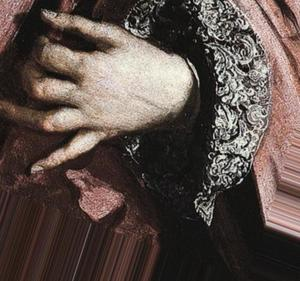
\includegraphics[width=0.170\textwidth]{figures/build/parts_example_2} &
        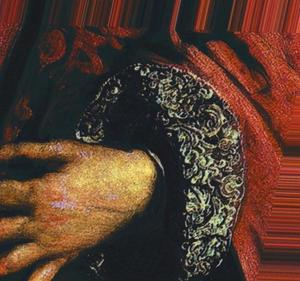
\includegraphics[width=0.170\textwidth]{figures/build/parts_example_18} &
        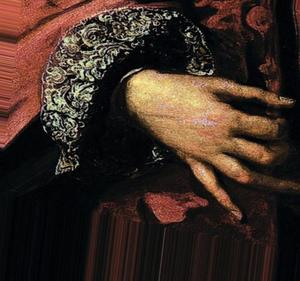
\includegraphics[width=0.170\textwidth]{figures/build/parts_example_19} &
        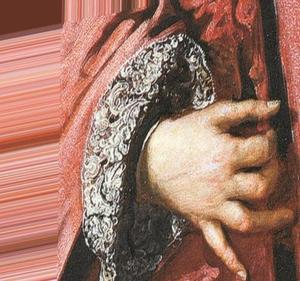
\includegraphics[width=0.170\textwidth]{figures/build/parts_example_5} \\

        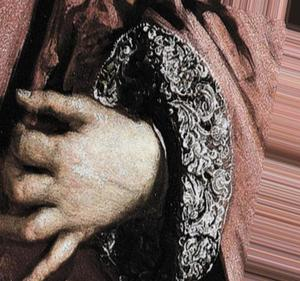
\includegraphics[width=0.170\textwidth]{figures/build/parts_example_6} &
        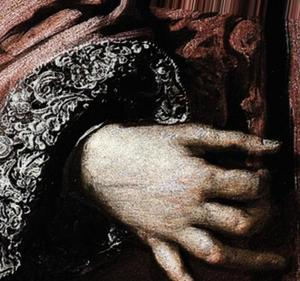
\includegraphics[width=0.170\textwidth]{figures/build/parts_example_7} &
        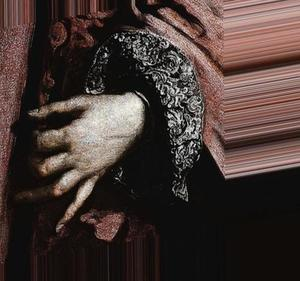
\includegraphics[width=0.170\textwidth]{figures/build/parts_example_8} &
        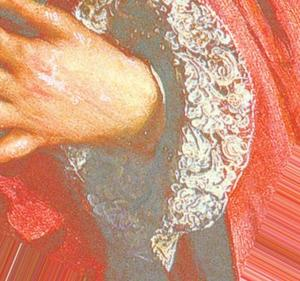
\includegraphics[width=0.170\textwidth]{figures/build/parts_example_9} &
        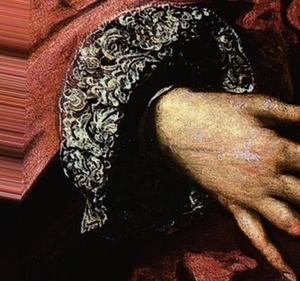
\includegraphics[width=0.170\textwidth]{figures/build/parts_example_10}
    \end{tabularx}
	\caption{Top-left is the original patch and the other ones are transformed samples}
    \label{fig:augmentation}
\end{figure}
As we will increasingly reduce the number of samples to train from data augmentation is immensely important. We subtract the mean of all images from the dataset from each training sample \citep{krizhevsky_imagenet_2012}. Moreover we employ multiple image transformations to artificially enlarge the trainings set. For this we use the preprocessing methods provided by the Keras library \citep{chollet_keras:_2015} and add additional transformations. Thus while training we generate new samples online with a set of bounded random transformations. The composite transformation $T_p$ is chosen with the random parameter vector $p = \{\alpha, \beta, s, t_x, t_y, m, t_s, t_v, f_s, f_v, v_s, v_v\}$ defining the following transformations:
\begin{my_list_item}
    \item \textbf{Rotation} with $\alpha\in[-\ang{20}, +\ang{20}]$
    \item \textbf{Shearing} with $\beta\in[-\ang{11.5}, + \ang{11.5}]$
    \item \textbf{Zoom} with $s\in[\SI{70}{\percent}, \SI{130}{\percent}]$
    \item \textbf{Translation} with $t_x,t_y\in[\SI{0}{\percent}, \SI{5}{\percent}]$ of the patches size in either directions on both axes.
    \item \textbf{Flipping} horizontally $m\in\{0,1\}$.
    \item \textbf{Contrast}. Patches are converted to the HSV color space. We raise saturation and value to a power $t_s, t_v \in [0.25, 4]$ then multiply by factors $f_s, f_v \in [0.7, 1.4]$ and add these to some values $v_s, v_v \in [-0.1, 0.1]$ \citep{dosovitskiy_discriminative_2014}. After the contrast transformation patches are again converted to RGB color space.
\end{my_list_item}
We set the parameter boundaries similar to those in \citet{dosovitskiy_discriminative_2014}.

Because the augmentation of training samples severely slows down training if done on demand we generate new samples in parallel to the network training.


\section{Generating detections}
\label{sec:pipeline:eval}
Our desired output of the algorithm is one or are multiple boxes enclosing each a section of the image which is predicted to contain the searched for type of object. The \gls{fcn} returns a score map as output. Each score predicts the probability of this pixel to be of the class we trained for. Therefore we need a method to return high scoring bounding boxes from a probability map. The here employed way of doing this consists of multiple steps:\\
\begin{my_list_num}
    \item We penalize (near-) empty regions inside the probability map with a negative distance transform
    \item We generate a set of boxes on a regular grid over the image shape
    \item For all those boxes we calculate their density of scores
    \item We apply a low threshold to filter out unnecessary boxes
    \item We apply \gls{nms} to get the top scoring boxes
\end{my_list_num}

\subsection{Negative Distance Transform}
\label{sec:pipeline:eval:dt}
\begin{figure}[htb]
    \begin{tabular}{ccc}
        A probability map & Thresholded map & Distance transform \\[3pt]
        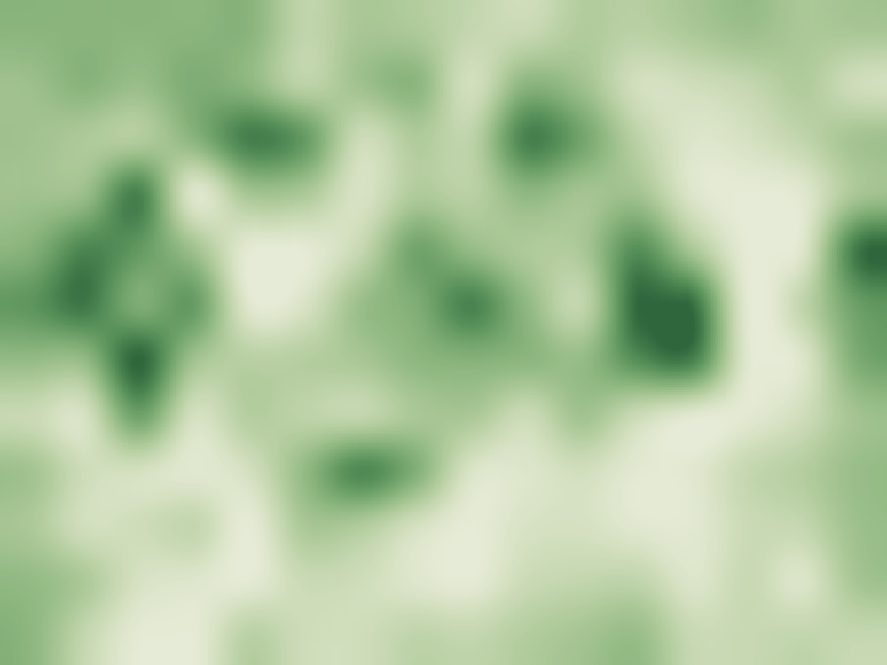
\includegraphics[width=0.303\textwidth]{figures/build/distance_transform_hm.pdf} &
        \includegraphics[width=0.303\textwidth]{figures/build/distance_transform_hm_thres-img0} &
        \includegraphics[width=0.303\textwidth]{figures/build/distance_transform_hm_negative-img0}
    \end{tabular}
	\caption{Computing the negative distance transform from an probability map}
    \label{fig:distance_transform}
\end{figure}
A lot of images produce probability maps that are sparsely filled. We want to penalize these uniform negative regions. Positive regions receive a positive score from the network while not-positive regions are at-most zero. Here we introduce a distance transform to score regions of near-zero values \fref{fig:distance_transform}.\\First we threshold the score map with a near-zero value to set all values that can safely assumed to be negatives to zero.\\Second we apply a distance transform to the mask that resulted from the thresholding. A distance transform fills each zero pixel of the mask with its distance to the nearest one valued pixel. The distances are calculated through some metric like the Euclidean distance or the $L_1$ distance. As the specific metric is not important for our vague penalizer and as we aim for good time performance we use the $L_\infty$ distance also known as the chessboard distance. For our 2-dimensional image space the metric is definde as follows:
\begin{equation}
    L_\infty = \max(|x_2 - x_1|, |y_2 - y_1|)
\end{equation}
The transformed image is normalized and substracted from the original probability map. This additional steps increases mean AUC on \textsc{Pascal}-Part by 3\%.

\subsection{Calculating the score densities}
\label{sec:pipeline:eval:density}
For each forwarded image we generate a set of boxes to calculate the score densities for. At three scales we take boxes $\{B_1,\dots B_i = (x_0, y_0, x_1, y_1)_i,\dots\}$ of the same aspect ratio as the input image and calculate the slices that would be the result of sliding the window over the image. Also we save the areas $\{A_1,\dots A_i,\dots\}$ of all rectangles.\\
Density is calculated by summing up all the probabilities from the score map inside each window and divided by the area of the window. To achieve that as efficiently as possible we use the integral image $I_\Sigma$ of our score map $I$. A value of the integral is the sum of all values left and above this point:
\begin{equation}
    I_\Sigma(x, y) = \sum_{\substack{x' \le x\\ y' \le y}} I(x', y')
\end{equation}
With the integral image the sum inside any rectangle of the image $I$ can then computed efficiently with:
\begin{equation}
    \sum_{\substack{x_0 < x \le x_1\\ y_0 < y \le y_1}}I(x,y) = I_\Sigma(x_1, y_1) + I_\Sigma(x_0, y_0) - I_\Sigma(x_1, y_0) - I_\Sigma(x_0, y_1)
\end{equation}

The probability density of each box is then computed through:
\begin{equation}
    \rho_i = \frac{\sum_{B_i}I(x,y)}{A_i}
\end{equation}

\subsection{Non maximum suppression}
\label{sec:pipeline:eval:nms}
\begin{figure}[htb]
    \begin{tabular}{ccc}
        Before \gls{nms} & After \gls{nms} \\[3pt]
        \includegraphics[width=0.47\textwidth]{figures/coypu} &
        \includegraphics[width=0.47\textwidth]{figures/coypu}
    \end{tabular}
	\caption{Computing the negative distance transform from an probability map}
    \label{fig:distance_transform}
\end{figure}
Depending on the number of scales we generate hundreds or even thousands of boxes per image. We want to eliminate boxes that are overlapping with another box that has a higher density. Firstly we drop the worst boxes $B_i: \rho_i < \rho_{min}$ with a low set threshold. While this is not necessary it greatly improves time performance and does not affect testing performance.\\To the remaining boxes we apply \gls{nms} as described by \citet{felzenszwalb_discriminatively_2008}. In the \gls{nms} we first sort all boxes by their descending scores which in our case are the probability densities. We mark the strongest box as picked. Then we calculate the area overlap between the new picked box and all remaining boxes. All boxes with an overlap in area of 0.5 or more are dropped. We pick the next strongest score of the remaining set and continue this process until all boxes are either dropped or picked. The strongest not-overlapping boxes remain picked and are returned. For minimal computational cost of this step we use the improved implementation from \citet{malisiewicz_ensemble_2011}.
